\documentclass[11pt,a4paper]{article}

\usepackage{latexsym}
\usepackage{graphicx}
\usepackage[french]{babel}


\usepackage{amsmath,amssymb}
\usepackage{pstricks,pst-plot}
\usepackage{calc}
\usepackage{multicol}
\usepackage{fancyhdr}
\usepackage{lastpage}
\usepackage[T1]{fontenc}
\usepackage[utf8]{inputenc}  
\usepackage{lmodern}
\usepackage{stmaryrd}
\usepackage[]{algorithm2e}
\usepackage{float}

\pagestyle{plain}

\title{DOVL : Assignment 1 \\ Stereo Matching with the $\alpha-\beta$ swap algorithm}
\author{Mathurin \textsc{Massias} \and Clément \textsc{Nicolle}}
\date{\today} 


\begin{document}
	
\maketitle

In order to speed up the algorithm, the labels were initialized using the unary terms. The initial label for pixel $p$ was selected as the $d \in \left[ 0, d_{max}\right] $ which minimizes $\mathcal{D}_p(l_p) = |I_{left}(y,x)-I_{right}(y,x-d)|$.

\begin{figure}[!htbp]
	\centering
	\noindent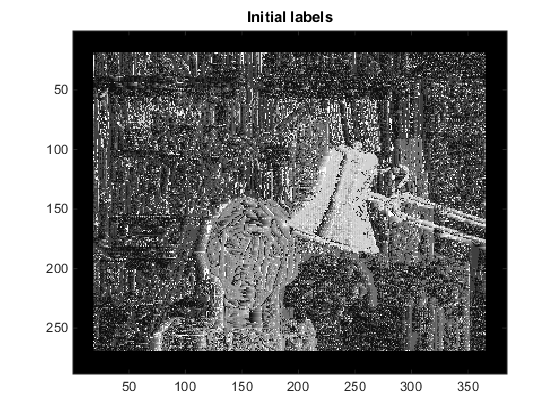
\includegraphics[scale=0.4]{results/initial_lab.png}
	\caption{Initial labeling}
\end{figure}

With parameters $K = 2$, $\lambda = 20$, $d_{max} = 15$, the algorithm converges, in term of energy, after 8 iterations, one iteration being all possible $\alpha-\beta$ swaps, with $\alpha \in \left[ 0, d_{max}-1\right] $ and $\beta \in \left[ \alpha+1, d_{max} \right] $

\begin{figure}[H]
	\centering
	\noindent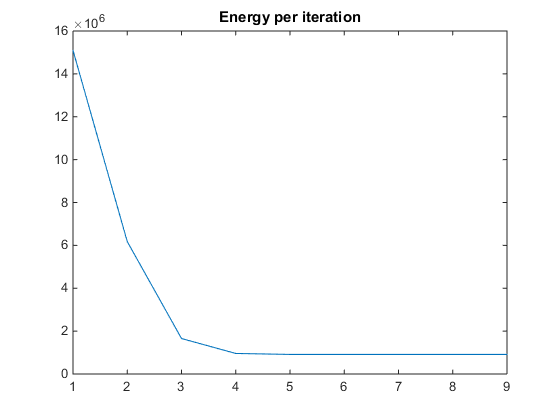
\includegraphics[scale=0.4]{results/energy.png}
	\caption{Energy at each iteration with $\lambda = 20$}
\end{figure}

\begin{figure}[H]
	\centering
	\noindent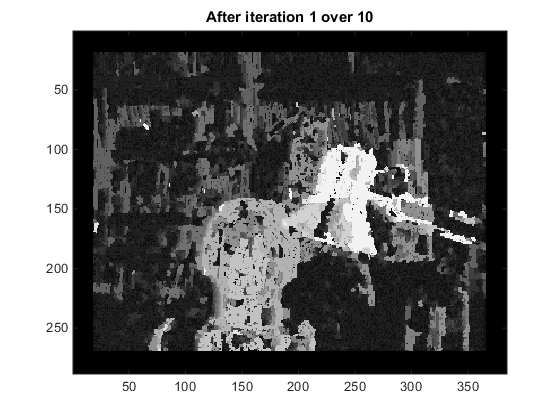
\includegraphics[scale=0.4]{results/one_iter.png}
	\noindent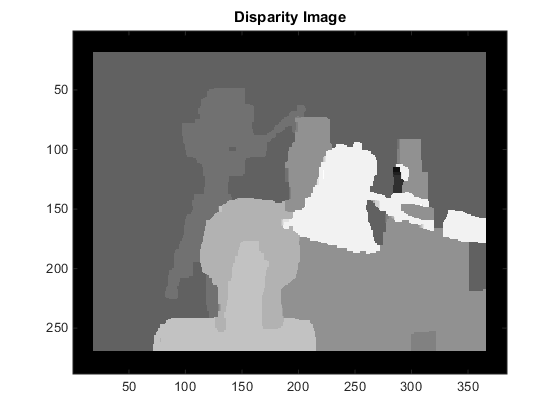
\includegraphics[scale=0.4]{results/disparity_est.png}
	\caption{Left : Depth map after one iteration - Right : Final depth map obtained with $\lambda = 20$}
\end{figure}

We were interested in analyzing the impact of the parameter $\lambda$. Intuitively, a higher $\lambda$ should give more importance to the pairwise terms and then result in a smoother depth map. Inversely, a smaller $\lambda$ should consider the details.
\\We tried $\lambda = 40$ and $\lambda = 10$. Both converged in 7 iterations, and our intuitions were confirmed, as you can see on the figures below.

\begin{figure}[H]
	\centering
	\noindent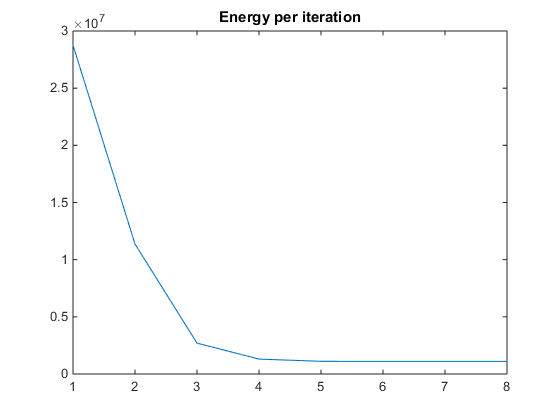
\includegraphics[scale=0.4]{results/energy40.png}
	\noindent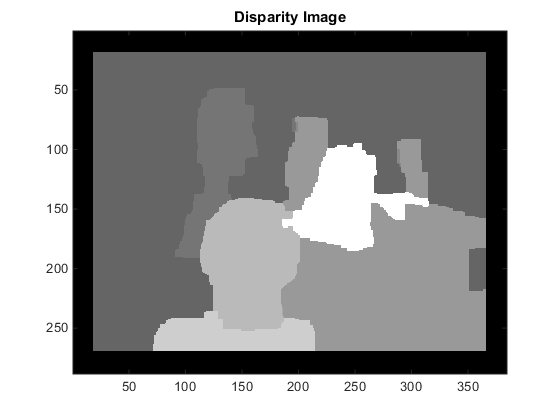
\includegraphics[scale=0.4]{results/disparity_est40-7it.png}
	\caption{Energy at each iteration and depth map obtained with $\lambda = 40$}
\end{figure}

\begin{figure}[H]
	\centering
	\noindent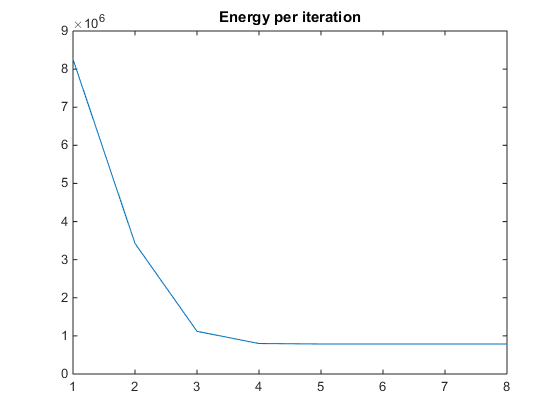
\includegraphics[scale=0.4]{results/energy10.png}
	\noindent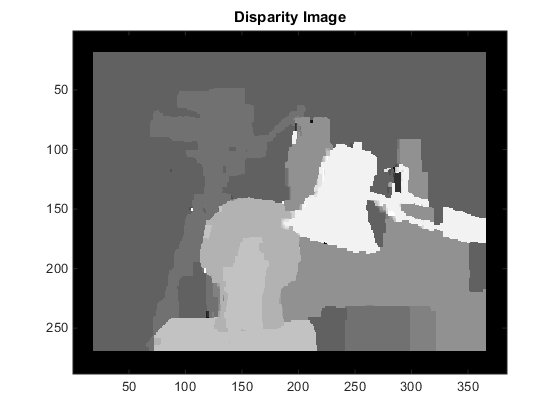
\includegraphics[scale=0.4]{results/disparity_est10-7it.png}
	\caption{Energy at each iteration and depth map obtained with $\lambda = 10$}
\end{figure}

\end{document}